\section{Wykorzystane oprogramowanie i biblioteki Pythona}

Pomijamy tutaj bibliotekę standardową jako wbudowaną w sam język, skupiając się na przydatnych bibliotekach zewnętrznych.

\subsection{Numpy}
\code{numpy}\cite{numpy} to biblioteka umożliwiająca wykonywanie złożonych obliczeń na
n-wymiarowych macierzach bądź tablicach, utworzona w celu umożliwienia
zastąpienia operacjami wektorowymi iteracji po tablicach, powszechnie
stosowanych w metodach numerycznych i będących znanym słabym punktem
Pythona.

Pod zewnętrzną powłoką zawiera odwołania do znanych, wypróbowanych i
sprawdzonych w nauce modułów \code{LAPACK}, \code{BLAS} napisanych w
szybkich, niskopoziomowych językach C oraz \code{FORTRAN}.  Jest to
\emph{de facto} standard większości obliczeń numerycznych w Pythonie.

Należy zauważyć, że operacje matematyczne w wersji \code{numpy} zawartej
w popularnej dystrybucji Anaconda są automatycznie zrównoleglane tam, gdzie
pozwala na to niezależność obliczeń dzięki dołączonym bibliotekom Intel Math
Kernel Library.\cite{intel-mkl} 

Numpy jest oprogramowaniem otwartym, udostępnianym na licencji BSD\@.


\subsection{scipy}
Kolejną podstawową biblioteką w numerycznym Pythonie jest \code{scipy}\cite{scipy},
biblioteka zawierająca wydajne gotowe implementacje wielu powszechnych algorytmów
numerycznych służących między innymi całkowaniu, optymalizacji funkcji rzeczywistych,
uczeniu maszynowemu, algebrze liniowej czy transformatom Fouriera.

\subsection{Numba}
\code{numba} to biblioteka służąca do kompilacji just-in-time wysokopoziomowego
kodu Pythona do kodu niskopoziomowego przy pierwszym uruchomieniu programu. W
wielu przypadkach pozwala na osiągnięcie kodem napisanym w czystym Pythonie
wydajności marginalnie niższej bądź nawet równej do analogicznego programu w C
bądź Fortranie.~\cite{numba}

Jednocześnie należy zaznaczyć prostotę jej użycia. W wielu przypadkach wystarczy
dodać do funkcji dekorator \code{@numba.jit}:

\lstinputlisting[language=Python, numbers=left, caption=Przykład zastosowania kompilacji just-in-time z biblioteki Numba wykorzystujący metody pomiaru czasu środowiska Jupyter.]{listings/numba_example.py}\label{lst:numba}

Istniejącym od niedawna kodem symulacyjnym implementującym tą metodę jest FBPIC\cite{fbpic}.


\subsection{HDF5}
HDF5 jest wysokowydajnym formatem plikow służącym przechowywaniu danych
liczbowych w drzewiastej, skompresowanej strukturze danych, razem z
równoległym, wielowątkowym zapisem tych danych.  W Pythonie implementuje go
biblioteka h5py\cite{h5py}.

W bieżącej pracy wykorzystuje się go do przechowywania danych liczbowych
dotyczących przebiegu symulacji, pozwalających na ich dalsze przetwarzanie
i analizę poprzez wizualizację.

\subsection{matplotlib}
Do wizualizacji danych z symulacji (oraz tworzenia schematów w sekcji
teoretycznej niniejszej pracy) użyto własnoręcznie napisanych skryptów w
uniwersalnej bibliotece graficznej \code{matplotlib}\cite{matplotlib}.
\code{matplotlib} zapewnia wsparcie zarówno dla grafik statycznych w różnych układach
współrzędnych (w tym 3D), jak również dla dynamicznie generowanych animacji
przedstawiających przebiegi czasowe symulacji.

\subsection{py.test}\label{sec:pytest}
Przy pracy nad kodem użyto frameworku testowego \code{py.test}~\cite{pytest}.
Tworzenie testów jest trywialne:

\lstinputlisting[language=Python, numbers=left, caption=Podstawowy przykład testu w pliku \code{func.py}]{listings/func.py}

Uruchamianie zaś:

\begin{lstlisting}[language=Bash]
    >>> pytest func.py
    === FAILURES ===
    ___failing ___

        def test_failing():
    >       assert f(4) == 13
    E       assert 12 == 13
    E        +  where 12 = f(4)

    func.py:10: AssertionError
    === 1 failed, 1 passed in 0.10 seconds ===
\end{lstlisting}

Należy zaznaczyć, że w symulacjach numerycznych, gdzie błędne działanie programu nie
objawia się zazwyczaj formalnym błędem, a jedynie błędnymi
wynikami, dobrze zautomatyzowane testy jednostkowe potrafią zaoszczędzić
bardzo dużo czasu na debugowaniu poprzez automatyzację uruchamiania
kolejnych partii kodu i lokalizację błędnie działających części algorytmu.
Dobrze napisane testy są praktycznie koniecznością w dzisiejszych czasach,
zaś każdy nowo powstały projekt symulacyjny powinien je
wykorzystywać, najlepiej do weryfikacji każdej części algorytmu z osobna.

Dobrym przykładem skutecznego testu jednostkowego jest porównanie energii kinetycznej
elektronu o znanej prędkości z wartością tablicową, zawarte jako test w pliku
\code{pythonpic/tests/test\_species.py}.

\code{py.test} jest oprogramowaniem otwartym, dostępnym na licencji MIT\@.

\subsection{Travis CI}
Nieocenionym narzędziem w pracy nad kodem był system ciągłej integracji
(\emph{continuous integration}) Travis CI~\cite{travisci}
dostępny za
darmo dla projektów open-source. Travis pobiera aktualne wersje kodu przy
każdej aktualizacji wersji dostępnej na serwerze GitHub i uruchamia testy,
zwracając komunikat o ewentualnym niepowodzeniu i pozwalając na jednoczesne
uruchamianie bieżących, intensywnych symulacji przy jednoczesnym
weryfikowaniu w chmurze poprawności działania lżejszych, acz wciąż intensywnych
symulacji testowych i testów algorytmicznych.

\subsection{snakeviz}

W optymalizacji przydatny okazał się program \code{snakeviz}\cite{snakeviz} dostępny na
GitHubie i pozwalający na wizualizację wyników z profilowania
symulacji. Pozwala w wygodny sposób zbadać, które fragmenty kodu najbardziej
spowalniają symulację, które są najlepszymi kandydatami do optymalizacji, oraz
jak skuteczne (bądź nieskuteczne) okazują się próby polepszenia ich wydajności.
Działanie programu ilustruje rysunek~\ref{fig:snakeviz}.
\begin{figure}[h!]
  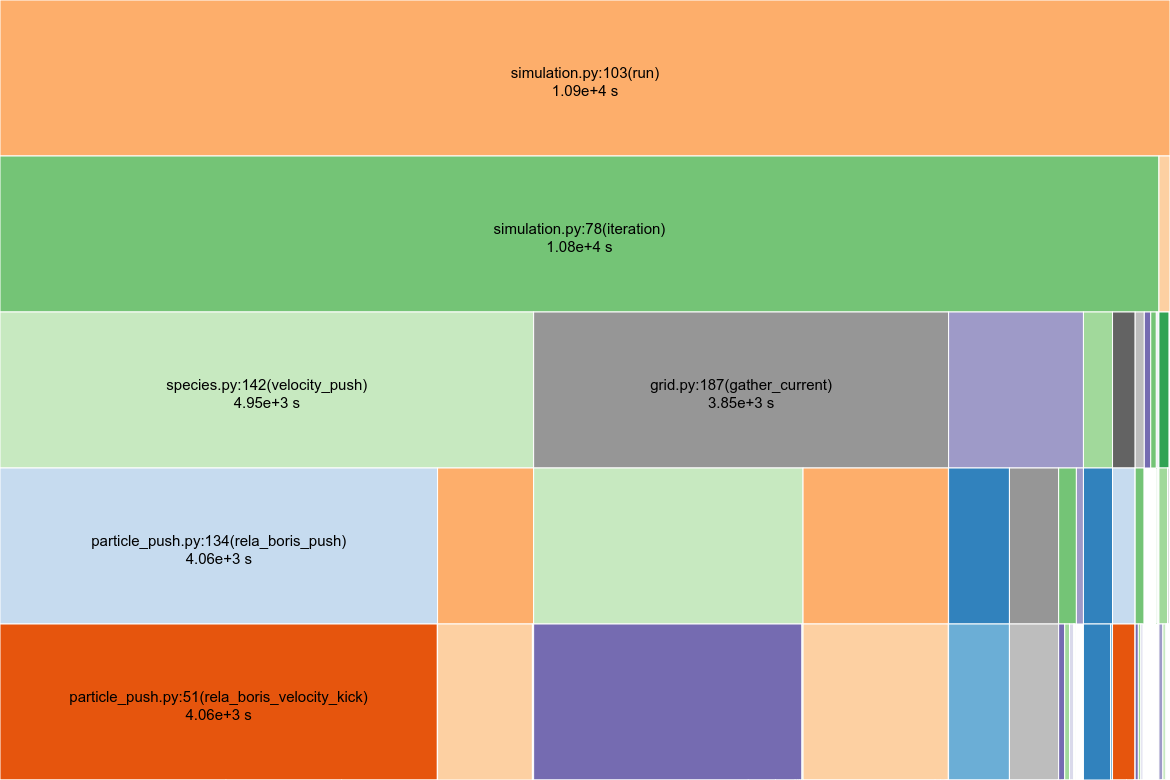
\includegraphics[width=\textwidth]{Images/snakeviz}
  \caption{Wizualizacja szybkości działania poszczególnych fragmentów kodu
    wygenerowana programem \code{snakeviz}.\label{fig:snakeviz}}
\end{figure}

\subsection{cProfile}
Uruchamianie kodu w celu zmierzenia wydajności całkowitej polegało na uruchomieniu skryptu \code{make benchmark}, który:
\begin{enumerate}
\item Czyści zawartość folderu \code{data\_analysis}, aby przeprowadzić obliczenia od początku bez wczytywania poprzednich danych
\item Uruchamia środowisko Anaconda zawierające bardziej zoptymalizowane od zwyczajnych wersje biblioteki Numpy
\item Uruchamia skrypt \code{fulllaser.py} w trybie \code{cProfile} i zapisuje dane do pliku \code{benchmark.prof}
\begin{lstlisting}[language=Bash]
   python -m cProfile -o benchmark.prof fulllaser.py
\end{lstlisting}
\end{enumerate}

Następnie zapisane dane są wizualizowane programem \code{snakeviz}.

Za wskaźnik efektów optymalizacji przyjęto całkowity czas trwania symulacji
oraz ułamek tego czasu spędzony w metodzie \code{iteration} klasy \code{Simulation}.
\subsection{IPython, \code{\%timeit}}
Do optymalizacji niewielkich fragmentów kodu wykorzystano środowisko Jupyter (dawniej IPython) Notebook\cite{jupyter}.
Użycie ``magicznych'' komend \code{\%timeit} pozwala na automatyczne profilowanie wydajności niewielkich fragmentów kodu.
Przykładem zastosowania tej komendy jest listing~\ref{lst:numba}.
